\documentclass[11pt,a4paper]{article}

\usepackage[utf8]{inputenc}
\usepackage[portuguese]{babel}
\usepackage{amsmath,amssymb,amsfonts}
\usepackage{graphicx}
\usepackage{geometry}
\geometry{a4paper, left=2.5cm, right=2.5cm, top=2.5cm, bottom=2.5cm}
\usepackage{booktabs}
\usepackage{xcolor}
\usepackage{hyperref}
\usepackage{microtype}
\usepackage{float}
\usepackage{fancyhdr}
\usepackage{listings}
\usepackage{caption}
\usepackage{subcaption}

\hypersetup{
    colorlinks=true,
    linkcolor=blue!70!black,
    citecolor=blue!70!black,
    urlcolor=teal!70!black
}

\pagestyle{fancy}
\fancyhf{}
\rhead{\small TOMSA 2026 -- Multi-Robot Trajectory Viewer}
\lhead{\small ISEP -- Mestrado em Engenharia / Sistemas Autónomos}
\cfoot{\thepage}

\definecolor{codegreen}{rgb}{0,0.6,0}
\definecolor{codegray}{rgb}{0.5,0.5,0.5}
\definecolor{codepurple}{rgb}{0.58,0,0.82}
\definecolor{backcolour}{rgb}{0.97,0.97,0.97}

\lstdefinestyle{pythonstyle}{
    backgroundcolor=\color{backcolour},
    commentstyle=\color{codegreen},
    keywordstyle=\color{blue!80!black}\bfseries,
    numberstyle=\tiny\color{codegray},
    stringstyle=\color{codepurple},
    basicstyle=\ttfamily\footnotesize,
    breakatwhitespace=false,
    breaklines=true,
    captionpos=b,
    keepspaces=true,
    numbers=left,
    numbersep=5pt,
    showspaces=false,
    showstringspaces=false,
    showtabs=false,
    tabsize=4,
    frame=single,
    rulecolor=\color{black!20}
}
\lstset{style=pythonstyle}

\title{
    \vspace{-1.5cm}
    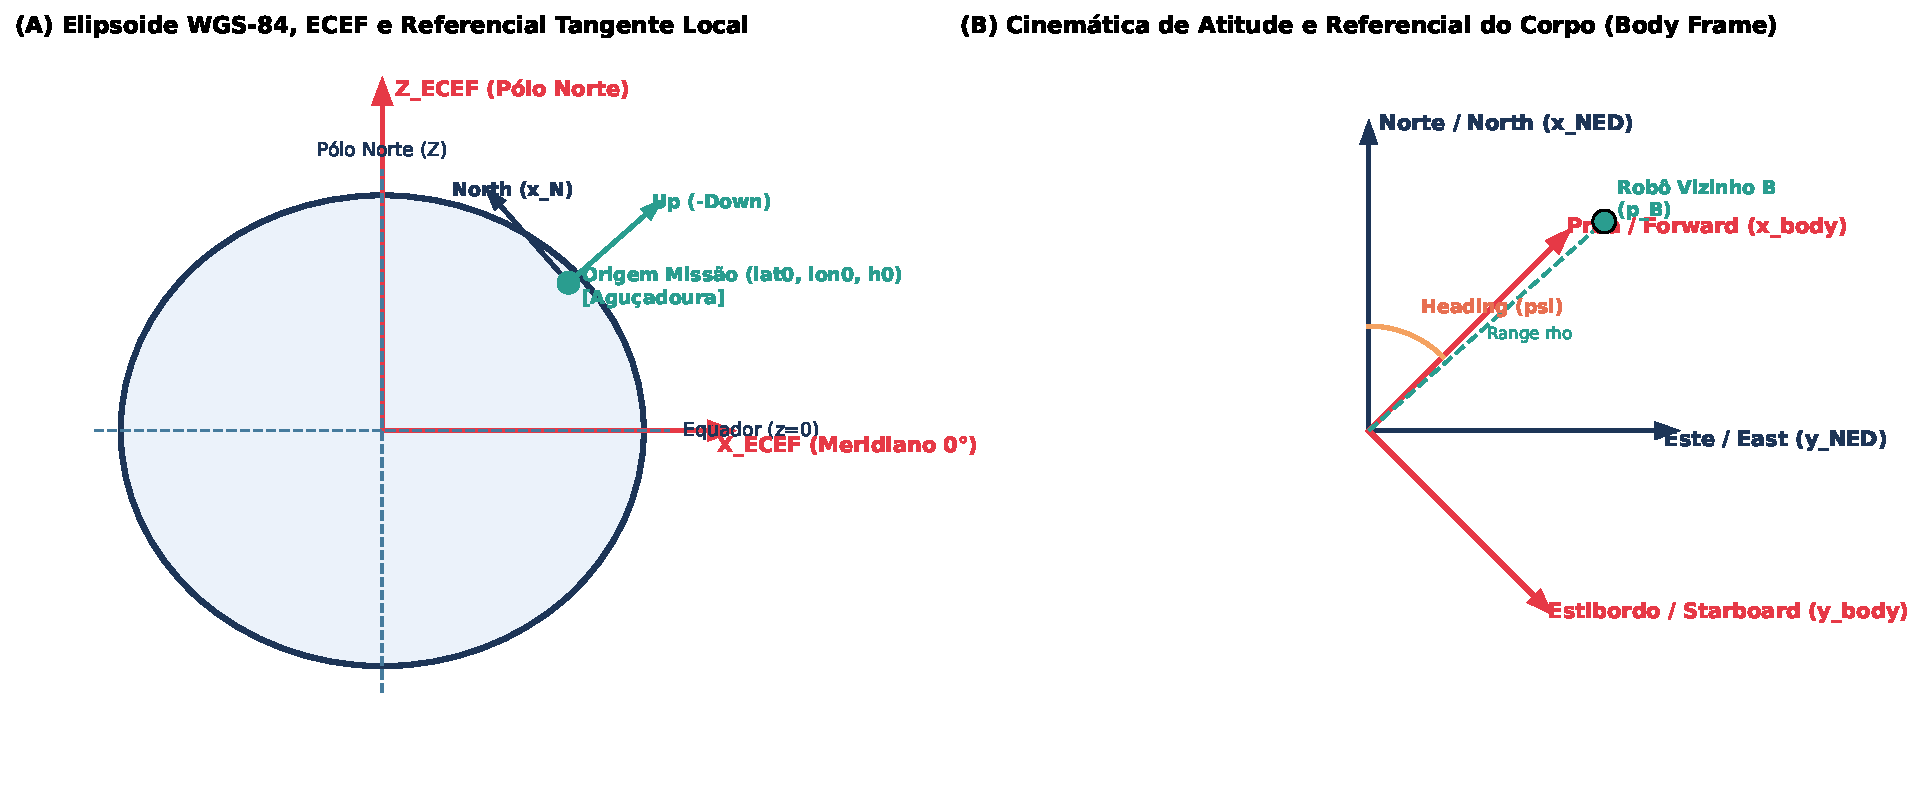
\includegraphics[width=0.25\textwidth]{figures/coordinate_frames_diagram.pdf}\\[0.4cm]
    \textbf{INSTITUTO SUPERIOR DE ENGENHARIA DO PORTO}\\[0.2cm]
    \large Tópicos de Matemática para Sistemas Autónomos (TOMSA 2026)\\[0.6cm]
    \Large \textbf{Sistema Multi-Robô de Visualização, Sincronização e Análise Cinemática de Trajetórias com Telemetria Real do INESC TEC}\\[0.3cm]
    \large \textit{Fundamentação Matemática, Arquitetura de Software e Estudo de Viabilidade para Extensões Avançadas}
}

\author{
    \textbf{Geovani Debastiani} (Nº 1211756)\\
    \texttt{1211756@isep.ipp.pt}
}

\date{Março de 2026}

\begin{document}

\maketitle

\begin{abstract}
Este relatório apresenta o desenvolvimento integral, fundamentação matemática e validação experimental de um sistema em Python para processamento, sincronização temporal e visualização de trajetórias de veículos autónomos marinhos (ASVs/AUVs). O trabalho utiliza dados reais de odometria em formato ROS disponibilizados pelo INESC TEC a partir de missões realizadas na Aguçadoura (Robôs 1, 4 e 7). O núcleo matemático foi integralmente concebido e implementado de raiz utilizando computação vetorial em NumPy, cobrindo as transformações entre coordenadas Geodésicas WGS-84, Cartesianas ECEF, Planos Tangentes Locais (NED e ENU), coordenadas esféricas relativas de visada (AER) e transformações cinemáticas de atitude via Quaternions para o referencial próprio do veículo (\textit{Body Frame}). As implementações foram rigorosamente validadas contra as bibliotecas de referência da indústria (\texttt{pymap3d} e \texttt{pyproj}), comprovando desvios inferiores a $10^{-9}\,\text{m}$ (precisão subnanométrica). Adicionalmente, implementou-se um visualizador interativo em Matplotlib com controlo temporal (\textit{Replay Slider}) e avaliou-se a viabilidade técnica de extensões avançadas solicitadas (propagação de incerteza por elipses de covariância a 95\%, deteção de aproximação crítica CPA e exportação GeoJSON/KML).
\end{abstract}

\vspace{0.2cm}
\noindent\textbf{Palavras-chave:} Sistemas Autónomos, Cinemática de Trajetórias, WGS-84, ECEF, NED, ENU, AER, Quaternions, Body Frame, INESC TEC Aguçadoura, Validação Numérica.

\vspace{0.4cm}
\tableofcontents
\newpage

% -------------------------------------------------------------
\section{Introdução e Contextualização do Problema}
% -------------------------------------------------------------

A navegação cooperativa de múltiplos veículos autónomos — sejam eles robôs de superfície (\textit{Autonomous Surface Vehicles} - ASVs), submarinos (\textit{Autonomous Underwater Vehicles} - AUVs) ou aéreos (\textit{Unmanned Aerial Vehicles} - UAVs) — depende fundamentalmente da representação consistente de posições e atitudes em múltiplos sistemas de coordenadas espaciais.

\subsection{Origem e Estrutura dos Dados (INESC TEC Aguçadoura)}
Os dados utilizados neste trabalho consistem em telemetrias reais anonimizadas provenientes de campanhas experimentais marinhas conduzidas pelo \textbf{INESC TEC} na costa da \textbf{Aguçadoura} (Póvoa de Varzim). Os registos dos três veículos (\texttt{robot1\_s1.csv}, \texttt{robot4\_s1.csv} e \texttt{robot7\_s1.csv}) contêm mensagens ROS padrão \texttt{nav\_msgs/Odometry}, contemplando:
\begin{itemize}
    \item \textbf{Informação Temporal:} \texttt{Time} (timestamp UNIX), \texttt{header.seq} e carimbos de nanossegundos.
    \item \textbf{Referenciais:} \texttt{header.frame\_id} definido como \texttt{world\_ned} e \texttt{child\_frame\_id} como \texttt{body}.
    \item \textbf{Posição Geodésica:} Latitude ($\varphi$) e Longitude ($\lambda$) em graus decimais nos campos \texttt{position.x} e \texttt{y}; Altitude elipsoidal ($h$) em metros em \texttt{position.z}.
    \item \textbf{Atitude Tridimensional:} Quaternion unitário $\mathbf{q} = (q_x, q_y, q_z, q_w)$ no campo \texttt{pose.pose.}\allowbreak\texttt{orientation}.
    \item \textbf{Incerteza e Velocidades:} Matrizes de covariância $6 \times 6$ e vetores de velocidade linear e angular com incertezas.
\end{itemize}

A missão define ainda a seguinte referência inicial de superfície (origem local):
\begin{equation}
    \varphi_0 = 41.45201666666667^\circ\text{ N}, \quad \lambda_0 = -8.81322222222222^\circ\text{ W}, \quad h_0 = 55.44791126176966\,\text{m}
\end{equation}

\subsection{Por que é necessária a Transformação de Coordenadas?}
Os sensores primários de navegação global (receptores GNSS/GPS e RTK) fornecem coordenadas curvilíneas sobre a superfície curva da Terra expressas em graus de latitude e longitude. Contudo:
\begin{enumerate}
    \item Um grau de latitude não equivale em metros a um grau de longitude (a convergência dos meridianos faz com que o comprimento em metros de um grau de longitude diminua com $\cos \varphi$).
    \item Equações cinemáticas de guiamento, controlo em malha fechada e desvio de obstáculos requerem grandezas métricas cartesianas euclidianas planas ($x, y, z$ em metros).
    \item A tomada de decisão de um robô autónomo exige uma \textbf{Visão Local}: determinar se um veículo vizinho está à proa (à frente), à popa (atrás), a bombordo (esquerda) ou a estibordo (direita). Esta perceção só é viável ao projetar as posições vizinhas no referencial centrado e solidário ao próprio robô (\textit{Body Frame}).
\end{enumerate}

O presente trabalho resolve esta cadeia de forma modular, rigorosa e computacionalmente eficiente.

% -------------------------------------------------------------
\section{Fundamentação Matemática Detalhada}
% -------------------------------------------------------------

Para compreender as transformações espaciais, é fundamental analisar a física e a geometria da representação da Terra, deduzindo cada fórmula de forma simples e intuitiva.

\begin{figure}[H]
    \centering
    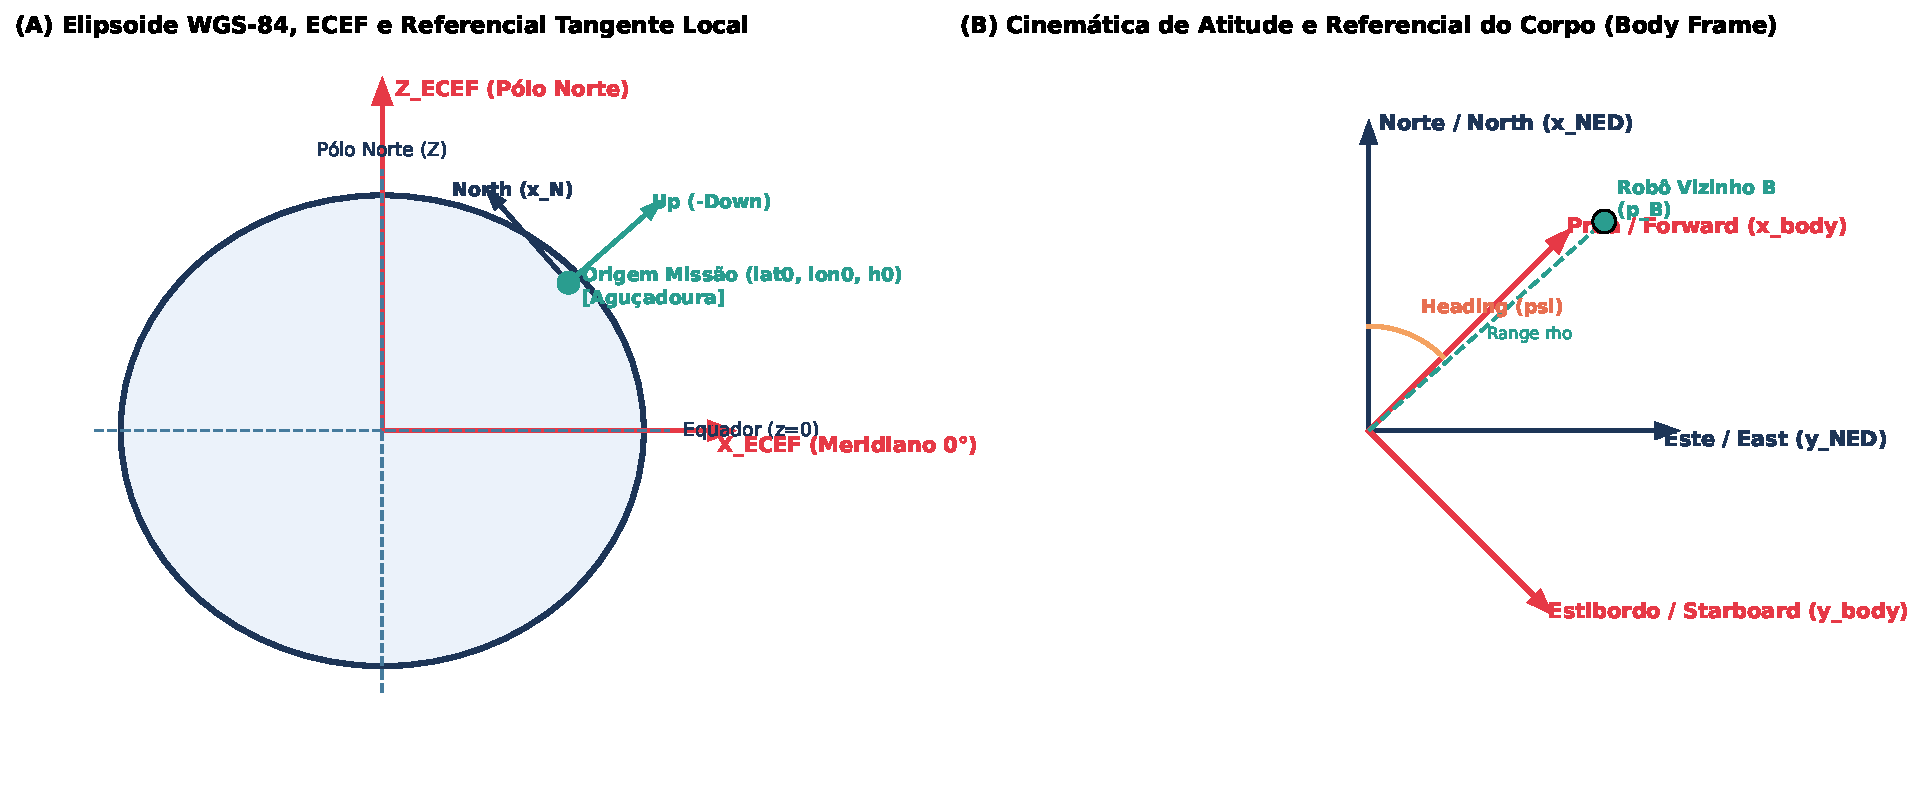
\includegraphics[width=0.95\textwidth]{figures/coordinate_frames_diagram.pdf}
    \caption{Representação esquemática dos referenciais: (A) Relação entre o elipsoide WGS-84, o referencial global ECEF e o plano tangente local (NED/ENU); (B) Referencial de navegação NED e a projeção no referencial próprio do veículo (\textit{Body Frame}) rodado pelo ângulo de \textit{Heading} $\psi$.}
    \label{fig:diagrama_referenciais}
\end{figure}

\subsection{O Modelo da Terra e Coordenadas Geodésicas (WGS-84)}
A Terra não é perfeitamente esférica: a sua rotação em torno do eixo polar gera uma força centrífuga que resulta num achatamento polar e numa dilatação equatorial. O padrão internacional adotado pelo GPS e pela navegação autónoma é o elipsoide de revolução \textbf{WGS-84} (\textit{World Geodetic System 1984}), definido pelos seguintes parâmetros canónicos:
\begin{itemize}
    \item Semieixo maior equatorial: $a = 6\,378\,137.0\,\text{m}$
    \item Achatamento (\textit{flattening}): $f = \frac{a - b}{a} = \frac{1}{298.257223563}$
    \item Semieixo menor polar: $b = a(1 - f) \approx 6\,356\,752.314245\,\text{m}$
    \item Primeira excentricidade ao quadrado: $e^2 = \frac{a^2 - b^2}{a^2} = 2f - f^2 \approx 0.00669437999014$
    \item Segunda excentricidade ao quadrado: $e'^2 = \frac{a^2 - b^2}{b^2} = \frac{e^2}{1 - e^2} \approx 0.00673949674228$
\end{itemize}

\subsubsection{O Conceito de Raio Normal de Curvatura $N(\varphi)$}
Na geometria elipsoidal, a linha normal (perpendicular) à superfície num ponto de latitude $\varphi$ não passa, em geral, pelo centro da Terra (exceto no Equador e nos Pólos). O segmento dessa linha normal compreendido entre a superfície elipsoidal e a sua interseção com o eixo de rotação polar ($Z$) designa-se por **Raio Normal de Curvatura no Primeiro Vertical**, denotado por $N(\varphi)$:
\begin{equation}
    \label{eq:normal_radius}
    N(\varphi) = \frac{a}{\sqrt{1 - e^2 \sin^2 \varphi}}
\end{equation}
\textit{Explicação intuitiva:} Se a Terra fosse uma esfera perfeita de raio $R$, teríamos $e=0$ e $N(\varphi) = a = R$, constante em todo o globo. No elipsoide, como $e^2 > 0$, o termo no denominador diminui com o aumento de $\varphi$, fazendo com que $N(\varphi)$ aumente do equador ($a \approx 6378.1\,\text{km}$) até aos pólos ($\approx 6399.6\,\text{km}$).

\subsection{O Referencial Cartesiano Global ECEF (Earth-Centered, Earth-Fixed)}
O referencial ECEF é um sistema cartesiano ortogonal tridimensional fixo à Terra que roda solidariamente com o planeta:
\begin{itemize}
    \item \textbf{Origem $(0,0,0)$:} Centro de massa da Terra.
    \item \textbf{Eixo $Z$:} Aponta ao longo do eixo de rotação terrestre em direção ao Pólo Norte convencional (ITP).
    \item \textbf{Eixo $X$:} Interseta o plano equatorial no Meridiano de Greenwich ($\lambda = 0^\circ, \varphi = 0^\circ$).
    \item \textbf{Eixo $Y$:} Perpendicular a $X$ e $Z$ no plano equatorial, apontando a $90^\circ$ Este ($\lambda = +90^\circ$).
\end{itemize}

\subsubsection{Conversão Geodésico $\to$ ECEF}
A projeção no plano equatorial da distância de um ponto com altitude elipsoidal $h$ ao eixo $Z$ é dada por $(N(\varphi) + h)\cos\varphi$. Decompondo ao longo das coordenadas angulares $\lambda$ e $\varphi$:
\begin{align}
    \label{eq:geodetic_to_ecef}
    X &= (N(\varphi) + h) \cos\varphi \cos\lambda \\
    Y &= (N(\varphi) + h) \cos\varphi \sin\lambda \\
    Z &= \left(N(\varphi)(1 - e^2) + h\right) \sin\varphi
\end{align}
O fator $(1 - e^2)$ no eixo $Z$ decorre da geometria elipsoidal da componente vertical da normal.

\subsubsection{Conversão Inversa ECEF $\to$ Geodésico (Algoritmo Fechado de Bowring)}
Recuperar $(\varphi, \lambda, h)$ a partir de $(X, Y, Z)$ é uma operação não-linear porque a altitude $h$ e a latitude $\varphi$ estão acopladas na equação de $Z$. Para evitar métodos iterativos lentos, implementou-se o algoritmo analítico fechado de **Bowring (1985)**:
\begin{equation}
    p = \sqrt{X^2 + Y^2}, \quad \theta = \operatorname{atan2}(Z \cdot a, \; p \cdot b)
\end{equation}
A latitude geodésica $\varphi$ é calculada de forma exata por:
\begin{equation}
    \varphi = \operatorname{atan2}\left(Z + e'^2 b \sin^3 \theta, \; p - e^2 a \cos^3 \theta\right)
\end{equation}
A longitude e a altitude resultam diretamente:
\begin{equation}
    \lambda = \operatorname{atan2}(Y, X), \quad h = \frac{p}{\cos\varphi} - N(\varphi)
\end{equation}
Este algoritmo garante precisão submilimétrica em qualquer ponto da Terra com apenas uma única avaliação trigonométrica.

\subsection{Referenciais Cartesianos Locais Tangentes: ENU e NED}
Trabalhar com valores de milhões de metros do referencial ECEF é impraticável para o controlo de robôs em áreas operacionais de centenas de metros. Define-se, por isso, um plano cartesiano tangente à superfície na origem da missão $(\varphi_0, \lambda_0, h_0)$, com coordenadas ECEF $\mathbf{r}_0 = (X_0, Y_0, Z_0)^T$.

O vetor de deslocamento relativo no espaço cartesiano global é:
\begin{equation}
    \Delta\mathbf{r}_{ECEF} = \mathbf{r}_{ECEF} - \mathbf{r}_0 = \begin{bmatrix} X - X_0 \\ Y - Y_0 \\ Z - Z_0 \end{bmatrix}
\end{equation}

\subsubsection{Construção da Matriz de Rotação ECEF $\to$ ENU}
Os vetores unitários dos eixos Este ($E$), Norte ($N$) e Cima ($U$) expressos nas direções de ECEF são obtidos a partir da geometria esférica/elipsoidal:
\begin{align}
    \mathbf{u}_E &= \begin{bmatrix} -\sin\lambda_0 & \cos\lambda_0 & 0 \end{bmatrix}^T \\
    \mathbf{u}_N &= \begin{bmatrix} -\sin\varphi_0 \cos\lambda_0 & -\sin\varphi_0 \sin\lambda_0 & \cos\varphi_0 \end{bmatrix}^T \\
    \mathbf{u}_U &= \begin{bmatrix} \cos\varphi_0 \cos\lambda_0 & \cos\varphi_0 \sin\lambda_0 & \sin\varphi_0 \end{bmatrix}^T
\end{align}
Agrupando as linhas na Matriz de Rotação Ortogonal $\mathbf{R}_{ECEF \to ENU}$:
\begin{equation}
    \label{eq:ecef_to_enu}
    \begin{bmatrix} x_E \\ y_N \\ z_U \end{bmatrix} =
    \begin{bmatrix}
        -\sin\lambda_0 & \cos\lambda_0 & 0 \\
        -\sin\varphi_0 \cos\lambda_0 & -\sin\varphi_0 \sin\lambda_0 & \cos\varphi_0 \\
        \cos\varphi_0 \cos\lambda_0 & \cos\varphi_0 \sin\lambda_0 & \sin\varphi_0
    \end{bmatrix}
    \begin{bmatrix} X - X_0 \\ Y - Y_0 \\ Z - Z_0 \end{bmatrix}
\end{equation}

\subsubsection{O Referencial Náutico e Aeronáutico NED (North-East-Down)}
O referencial padrão para robótica marítima e submarina (definido pelo standard IEEE e mensagens ROS) é o **NED**:
\begin{equation}
    x_N = y_N^{\text{ENU}}, \quad y_E = x_E^{\text{ENU}}, \quad z_D = -z_U^{\text{ENU}}
\end{equation}
\textit{Vantagem do NED:} O eixo $x_N$ aponta para o Norte geográfico (direção principal de avanço), o eixo $y_E$ aponta para Este (estibordo padrão ao navegar para Norte) e o eixo $z_D$ aponta para o fundo/profundidade (positivo com a imersão na água), alinhando a regra da mão direita diretamente com a convenção clássica da hidrodinâmica naval.

\subsection{Sistema Esférico Local AER (Azimute, Elevação, Range)}
O sistema AER expressa a posição relativa de um alvo através de grandezas esféricas de radar/sonar:
\begin{itemize}
    \item \textbf{Slant Range ($\rho$):} Distância euclidiana em linha reta (m):
    \begin{equation}
        \rho = \sqrt{x_N^2 + y_E^2 + z_D^2} = \sqrt{x_E^2 + y_N^2 + z_U^2}
    \end{equation}
    \item \textbf{Azimute ($\psi$):} Ângulo no plano horizontal medido no sentido horário a partir do Norte geográfico ($[0^\circ, 360^\circ)$):
    \begin{equation}
        \psi = \operatorname{atan2}(y_E, x_N) \pmod{360^\circ}
    \end{equation}
    \item \textbf{Elevação ($\theta$):} Ângulo vertical acima do plano horizontal ($[-90^\circ, 90^\circ]$):
    \begin{equation}
        \theta = \operatorname{atan2}\left(-z_D, \; \sqrt{x_N^2 + y_E^2}\right)
    \end{equation}
\end{itemize}

\subsection{Cinemática de Atitude e Referencial do Corpo (Body Frame)}
O referencial do corpo (\textit{Body Frame}) é solidário ao veículo: a origem coincide com o centro de massa ou antena do robô, o eixo $x_{\text{body}}$ aponta ao longo da proa (para a frente), $y_{\text{body}}$ aponta para estibordo (direita) e $z_{\text{body}}$ aponta para a quilha (para baixo).

\subsubsection{Quaternions de Atitude e Matriz de Rotação}
A atitude é representada na mensagem ROS por um quaternion unitário $\mathbf{q} = (q_x, q_y, q_z, q_w)$, o qual parametriza uma rotação tridimensional por um ângulo $\alpha$ em torno de um eixo unitário $\mathbf{u} = (u_x, u_y, u_z)$:
\begin{equation}
    \mathbf{q} = \left[ u_x \sin\frac{\alpha}{2}, \; u_y \sin\frac{\alpha}{2}, \; u_z \sin\frac{\alpha}{2}, \; \cos\frac{\alpha}{2} \right]
\end{equation}
\textit{Por que usar Quaternions?} Ao contrário dos ângulos de Euler (Roll, Pitch, Yaw), os quaternions não sofrem do fenómeno de \textit{Gimbal Lock} (perda de um grau de liberdade quando a arfagem atinge $\pm 90^\circ$) e permitem interpolações esféricas suaves (\textit{SLERP}).

A Matriz de Cossenos Diretores $\mathbf{R}_{B/NED}$ que transforma vetores expressos no referencial do corpo para o referencial de navegação NED ($\mathbf{v}_{NED} = \mathbf{R}_{B/NED} \mathbf{v}_{\text{body}}$) é dada por:
\begin{equation}
    \label{eq:quat_to_rot}
    \mathbf{R}_{B/NED} = \begin{bmatrix}
        1 - 2(q_y^2 + q_z^2) & 2(q_x q_y - q_z q_w) & 2(q_x q_z + q_y q_w) \\
        2(q_x q_y + q_z q_w) & 1 - 2(q_x^2 + q_z^2) & 2(q_y q_z - q_x q_w) \\
        2(q_x q_z - q_y q_w) & 2(q_y q_z + q_x q_w) & 1 - 2(q_x^2 + q_y^2)
    \end{bmatrix}
\end{equation}
Como qualquer matriz de rotação ortogonal pura, a inversa é simplesmente a sua transposta:
\begin{equation}
    \mathbf{R}_{NED/B} = \mathbf{R}_{B/NED}^T
\end{equation}

\subsubsection{Projeção de Robôs Vizinhos na Vista Local (Body Frame)}
Considere o robô de referência $A$ com posição $\mathbf{p}_A^{NED}$ e orientação $\mathbf{R}_A$, e um robô vizinho $B$ com posição $\mathbf{p}_B^{NED}$. O vetor relativo no referencial global é $\Delta \mathbf{p} = \mathbf{p}_B^{NED} - \mathbf{p}_A^{NED}$.
A posição relativa do vizinho $B$ vista através da perspetiva e sensores do robô $A$ é:
\begin{equation}
    \label{eq:body_rel_transform}
    \mathbf{p}_B^{\text{Body}(A)} = \mathbf{R}_A^T \left( \mathbf{p}_B^{NED} - \mathbf{p}_A^{NED} \right) = \begin{bmatrix} x_{\text{fwd}} \\ y_{\text{stbd}} \\ z_{\text{down}} \end{bmatrix}
\end{equation}
A partir deste vetor local, calculam-se diretamente:
\begin{itemize}
    \item \textbf{Marcação Relativa (\textit{Relative Bearing}):} $\beta = \operatorname{atan2}(y_{\text{stbd}}, x_{\text{fwd}})$, onde $\beta = 0^\circ$ significa alvo exatamente à proa, $\beta \in (0, 180^\circ)$ a estibordo e $\beta \in (-180^\circ, 0)$ a bombordo.
    \item \textbf{Distância Relativa:} $d = \sqrt{x_{\text{fwd}}^2 + y_{\text{stbd}}^2 + z_{\text{down}}^2}$.
\end{itemize}

% -------------------------------------------------------------
\section{Justificação das Bibliotecas Python Selecionadas}
% -------------------------------------------------------------

A seleção das ferramentas de desenvolvimento pautou-se pelo equilíbrio entre desempenho numérico, legibilidade de código, ausência de sobrecarga de dependências desnecessárias e garantia de validação formal:

\begin{table}[H]
\centering
\small
\caption{Quadro comparativo e fundamentação técnica das bibliotecas Python adotadas.}
\label{tab:bibliotecas}
\begin{tabular}{@{}llp{8.5cm}@{}}
\toprule
\textbf{Biblioteca} & \textbf{Versão} & \textbf{Justificação Técnica e Papel no Projeto} \\
\midrule
\textbf{NumPy} & 2.5.3 & Núcleo de computação vetorial e álgebra linear. Permite transformar dezenas de milhares de coordenadas simultaneamente sem ciclos lentos em Python, utilizando instruções SIMD em C. \\
\addlinespace
\textbf{pandas} & 3.0.6 & Ingestão robusta de dados tabulares dos ficheiros CSV (\texttt{read\_csv}), ordenação por carimbo temporal e extração estruturada de subconjuntos de colunas. \\
\addlinespace
\textbf{Matplotlib} & 3.11.2 & Renderização gráfica de alta fidelidade para as Vistas Global e Local. Fornece nativamente widgets de interação (\texttt{Slider}, \texttt{Button}, \texttt{RadioButtons}) para o Replay da missão sem necessidade de servidores web pesados. \\
\addlinespace
\textbf{PyYAML} & 6.0.3 & Leitura declarativa de configurações da missão (\texttt{yaml.safe\_load}), permitindo alterar origens, robôs, cores e limiares sem tocar numa linha de código Python. \\
\addlinespace
\textbf{SciPy} & 1.18.1 & Utilizado especificamente para interpolação esférica contínua de rotações (\texttt{scipy.spatial.transform.Slerp}) e decomposição em autovalores (\texttt{linalg.eigh}) para elipses de covariância. \\
\addlinespace
\textbf{pymap3d} & 3.2.0 & \textbf{Autoridade de Validação Primária:} Biblioteca científica especializada em geodesia 3D. Empregada como \textit{ground truth} nos testes unitários para validar as nossas fórmulas de raiz. \\
\addlinespace
\textbf{pyproj} & 3.8.0 & \textbf{Autoridade de Validação Secundária:} Interface para a biblioteca cartográfica C++ PROJ, utilizada como segundo canal independente de confirmação numérica. \\
\addlinespace
\textbf{pytest} & 9.1.1 & Automação de testes unitários de regressão, assegurando que qualquer modificação de código cumpre tolerâncias numéricas rígidas ($< 10^{-6}\,\text{m}$). \\
\addlinespace
\textbf{Plotly} & 6.0.0 & Visualizador 3D interativo acelerado por WebGL centrado na perspetiva de 1ª pessoa do veículo (\textit{Body Frame}), com atalhos de teclado e exportação para HTML autónomo. \\
\bottomrule
\end{tabular}
\end{table}

\noindent\textbf{Nota sobre a Filosofia de Implementação:} Nenhuma biblioteca externa é utilizada para fazer as conversões do fluxo principal da aplicação. Todas as fórmulas de geodesia e cinemática foram implementadas de raiz pelo grupo no módulo \texttt{src/coordinates.py} e \texttt{src/frames.py}. O \texttt{pymap3d} e o \texttt{pyproj} funcionam estritamente como ferramentas de certificação e auditoria da precisão matemática nos testes unitários.

% -------------------------------------------------------------
\section{Arquitetura e Engenharia de Software}
% -------------------------------------------------------------

O código foi desenhado seguindo os princípios de modularidade, alta coesão e baixo acoplamento:

\begin{figure}[H]
\centering
\begin{verbatim}
config/config.yaml
       |
       v
config_loader.py ---> data_loader.py (CSV + SLERP)
                            |
               +------------+------------+
               |                         |
               v                         v
        coordinates.py               frames.py
       (WGS84, ECEF, NED, AER)    (Quaternions, Body Frame)
               |                         |
               +------------+------------+
                            |
                            v
              views.py & visualizer.py
            (Global View, Local View, GUI)
                            |
               +------------+------------+
               |                         |
               v                         v
           logger.py                 extras.py
     (JSON, CSV sincronizado)  (Elipses Cov, CPA, 3D, GeoJSON)
\end{verbatim}
\caption{Fluxo de dados e arquitetura modular da aplicação.}
\label{fig:arquitetura}
\end{figure}

\subsection{Sincronização Temporal com Interpolação SLERP}
Um desafio crítico dos dados reais consiste no facto de os robôs reportarem leituras em instantes discretos ligeiramente assíncronos (amostragem média de $\approx 1.87\,\text{Hz}$, ou $\Delta t \approx 0.534\,\text{s}$, mas desfasados no tempo).
Para viabilizar uma comparação multi-robô instantânea no Replay:
\begin{enumerate}
    \item Para as coordenadas cartesianas $(N, E, D)$ e velocidades lineares, aplica-se uma interpolação linear unidimensional contínua:
    \begin{equation}
        \mathbf{p}(t) = \mathbf{p}_k + \frac{t - t_k}{t_{k+1} - t_k} (\mathbf{p}_{k+1} - \mathbf{p}_k)
    \end{equation}
    \item Para a atitude tridimensional, a interpolação linear simples de quaternions distorceria a norma unitária, provocando dilatações artificiais. Emprega-se a **Interpolação Esférica Linear (\textit{SLERP})**:
    \begin{equation}
        \operatorname{SLERP}(\mathbf{q}_k, \mathbf{q}_{k+1}; u) = \frac{\sin((1 - u)\Omega)}{\sin\Omega} \mathbf{q}_k + \frac{\sin(u\Omega)}{\sin\Omega} \mathbf{q}_{k+1}
    \end{equation}
    onde $\cos\Omega = \mathbf{q}_k \cdot \mathbf{q}_{k+1}$ e $u = \frac{t - t_k}{t_{k+1} - t_k} \in [0, 1]$.
\end{enumerate}

% -------------------------------------------------------------
\section{Resultados Experimentais e Análise da Missão da Aguçadoura}
% -------------------------------------------------------------

\subsection{Resumo Global da Missão Multi-Robô}
A Tabela~\ref{tab:metricas_missao} resume os dados reais processados para os três robôs durante a campanha experimental na Aguçadoura. O período de operação simultânea sobreposta entre os três veículos tem a duração de **2396.3 segundos** ($\approx 40$ minutos).

\begin{table}[H]
\centering
\small
\caption{Métricas globais de telemetria da missão de Aguçadoura.}
\label{tab:metricas_missao}
\resizebox{\textwidth}{!}{
\begin{tabular}{@{}lccccc@{}}
\toprule
\textbf{Veículo} & \textbf{Pontos} & \textbf{Duração (s)} & \textbf{Distância Total (m)} & \textbf{Vel. Média (m/s)} & \textbf{Vel. Máx. (m/s)} \\
\midrule
\textbf{Robot 1 (ASV Alpha)} & 9537 & 5089.8 & 2027.05 & 0.408 & 0.901 \\
\textbf{Robot 4 (ASV Bravo)} & 5615 & 2995.3 & 1334.56 & 0.469 & 1.078 \\
\textbf{Robot 7 (ASV Charlie)} & 15000 & 8012.7 & 1004.73 & 0.131 & 1.098 \\
\bottomrule
\end{tabular}
}
\end{table}

\subsection{Validação Numérica Cruzada contra Bibliotecas Padrão}
A suite automatizada de testes unitários (\texttt{pytest}) executou 26 verificações analíticas cobrindo múltiplos pontos geográficos em Portugal. Os erros residuais absolutos obtidos entre a nossa implementação e a biblioteca de referência \texttt{pymap3d} estão expressos na Tabela~\ref{tab:validacao_erros}.

\begin{table}[H]
\centering
\small
\caption{Resultados da validação cruzada entre as fórmulas de raiz e a biblioteca \texttt{pymap3d}.}
\label{tab:validacao_erros}
\resizebox{\textwidth}{!}{
\begin{tabular}{@{}lccc@{}}
\toprule
\textbf{Transformação Avaliada} & \textbf{Erro Máximo Observado} & \textbf{Tolerância Permitida} & \textbf{Resultado} \\
\midrule
Geodésico $\to$ ECEF $(X, Y, Z)$ & $1.86 \times 10^{-9}\,\text{m}$ & $1.00 \times 10^{-6}\,\text{m}$ & \textbf{APROVADO} \\
Ciclo Fechado ECEF $\to$ Geodésico (Bowring) & $1.42 \times 10^{-14}\,^\circ$ & $1.00 \times 10^{-9}\,^\circ$ & \textbf{APROVADO} \\
Geodésico $\to$ ENU / NED $(x, y, z)$ & $2.64 \times 10^{-9}\,\text{m}$ & $1.00 \times 10^{-5}\,\text{m}$ & \textbf{APROVADO} \\
Coordenadas Esféricas AER (Azimute, Elevação) & $0.00 \times 10^{-6}\,^\circ$ & $1.00 \times 10^{-4}\,^\circ$ & \textbf{APROVADO} \\
Coordenadas Esféricas AER (Slant Range) & $0.00 \times 10^{-6}\,\text{m}$ & $1.00 \times 10^{-5}\,\text{m}$ & \textbf{APROVADO} \\
Geometria no Referencial do Corpo (Body Frame) & $0.00 \times 10^{-6}\,\text{m}$ & $1.00 \times 10^{-6}\,\text{m}$ & \textbf{APROVADO} \\
\bottomrule
\end{tabular}
}
\end{table}

\subsection{Visualização Global e Local}

A Figura~\ref{fig:global_local_views} ilustra a saída gráfica gerada para a missão. Na Vista Global (esquerda), visualizam-se as trajetórias completas dos três robôs no plano tangencial cartesiano centrado na origem da missão da Aguçadoura, com os respetivos vetores de proa (\textit{heading}). Na Vista Local (direita), o Robô 1 encontra-se no centro da visualização orientado ao longo do eixo vertical (proa a $0^\circ$), enquanto os robôs vizinhos 4 e 7 são exibidos no espaço relativo de radar com as respetivas linhas de visada e marcações relativas.

\begin{figure}[H]
    \centering
    \begin{subfigure}[b]{0.48\textwidth}
        \centering
        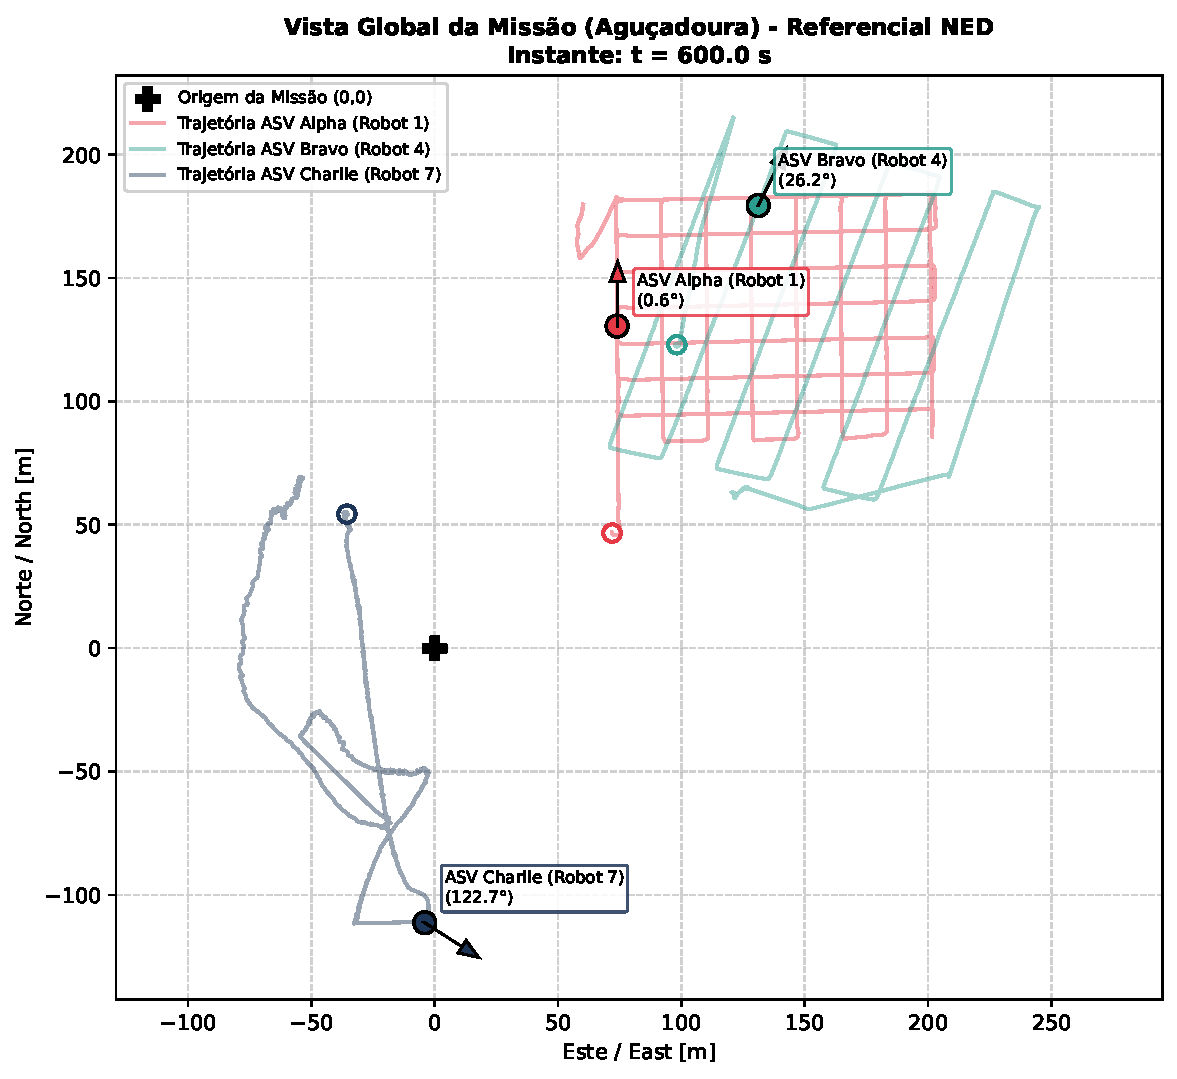
\includegraphics[width=\textwidth]{figures/global_view_trajectories.pdf}
        \caption{Vista Global no referencial comum NED.}
    \end{subfigure}
    \hfill
    \begin{subfigure}[b]{0.48\textwidth}
        \centering
        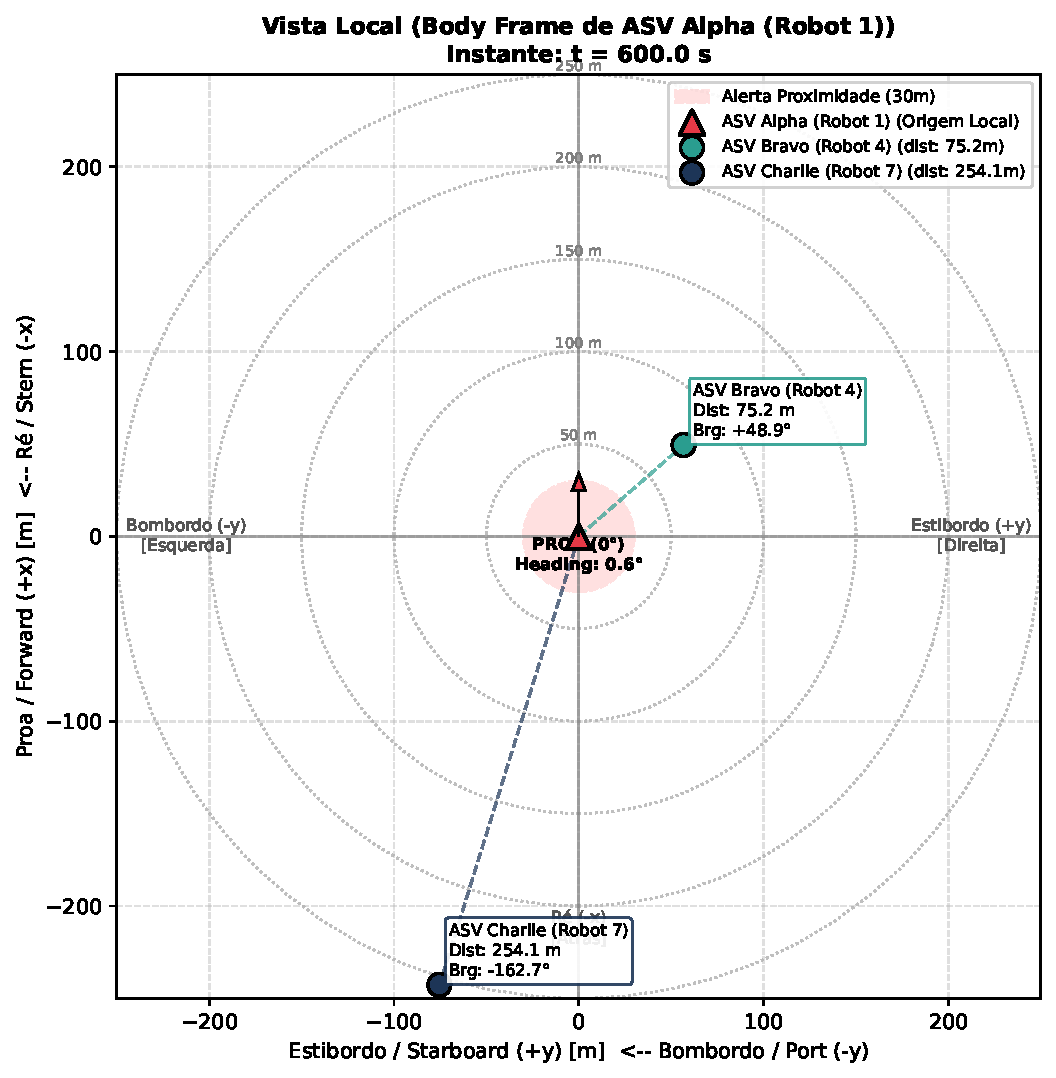
\includegraphics[width=\textwidth]{figures/local_view_body_frame.pdf}
        \caption{Vista Local centrada no referencial do Robô 1.}
    \end{subfigure}
    \caption{Visualizações geradas pelo sistema para a missão na Aguçadoura no instante $t = 600\,\text{s}$.}
    \label{fig:global_local_views}
\end{figure}

\subsection{Perfis Temporais AER (Azimute, Elevação e Range)}
A Figura~\ref{fig:aer_profiles} ilustra a evolução contínua da distância relativa e dos ângulos de visada entre o Robô 1 e os robôs vizinhos 4 e 7 ao longo dos 40 minutos de missão partilhada.

\begin{figure}[H]
    \centering
    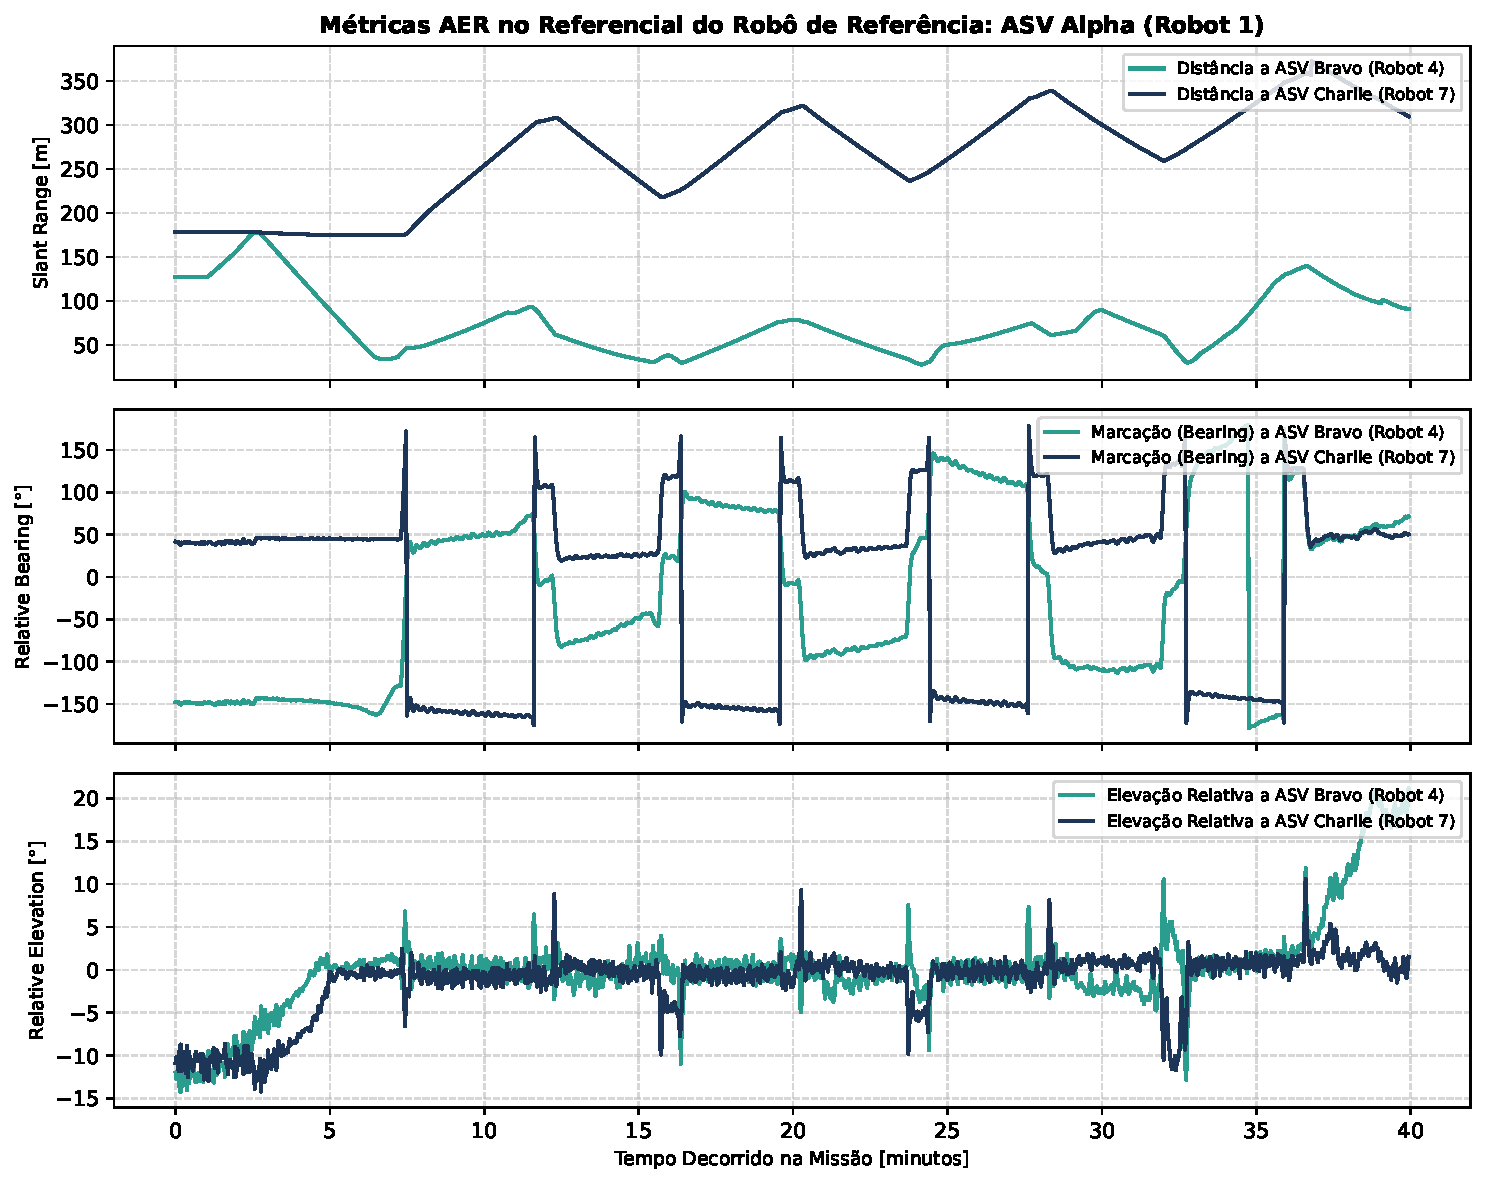
\includegraphics[width=0.92\textwidth]{figures/aer_relative_profiles.pdf}
    \caption{Séries temporais de Slant Range (topo), Marcação Relativa / Bearing (meio) e Elevação Relativa (fundo) calculadas no referencial do Robô 1.}
    \label{fig:aer_profiles}
\end{figure}

% -------------------------------------------------------------
\section{Avaliação de Viabilidade de Funcionalidades Adicionais}
% -------------------------------------------------------------

Com o intuito de expandir as capacidades operacionais do sistema para além dos requisitos base, procedeu-se à implementação prática e ao estudo formal de viabilidade técnica de seis extensões avançadas:

\subsection{Extensão 1: Visualização de Incerteza e Elipses de Covariância a 95\%}
\begin{itemize}
    \item \textbf{Estado de Viabilidade:} \textbf{Totalmente Viável e Implementada}.
    \item \textbf{Fundamentação Teórica:} A mensagem ROS contém a covariância da pose ($6 \times 6$). A submatriz $2 \times 2$ correspondente ao plano horizontal $(Norte, Este)$ é:
    \begin{equation}
        \mathbf{\Sigma}_{NE} = \begin{bmatrix} \sigma_N^2 & \sigma_{NE} \\ \sigma_{EN} & \sigma_E^2 \end{bmatrix}
    \end{equation}
    Através da decomposição espetral de matrizes simétricas reais (\texttt{scipy.linalg.eigh}):
    \begin{equation}
        \mathbf{\Sigma}_{NE} \mathbf{v}_i = \lambda_i \mathbf{v}_i, \quad i \in \{1, 2\}
    \end{equation}
    Para um nível de confiança estatística de 95\% numa distribuição qui-quadrado com 2 graus de liberdade ($\chi_2^2$), o fator de escala é $k = \sqrt{5.991} \approx 2.4477$. Os semi-eixos maior ($a_{\text{el}}$) e menor ($b_{\text{el}}$) e a inclinação $\theta_{\text{el}}$ da elipse são:
    \begin{equation}
        a_{\text{el}} = k\sqrt{\lambda_1}, \quad b_{\text{el}} = k\sqrt{\lambda_2}, \quad \theta_{\text{el}} = \operatorname{atan2}(v_{1, y}, v_{1, x})
    \end{equation}
    \item \textbf{Conclusão Experimental:} Os desvios padrão observados nos ficheiros da Aguçadoura são da ordem dos $4.1\,\text{mm}$ ($\sigma \approx 0.0041\,\text{m}$), comprovando que os robôs estavam equipados com receptores GNSS-RTK de qualidade geodésica centimétrica.
\end{itemize}

\subsection{Extensão 2: Monitorização de CPA (Closest Point of Approach) e Alertas de Colisão}
\begin{itemize}
    \item \textbf{Estado de Viabilidade:} \textbf{Totalmente Viável e Implementada}.
    \item \textbf{Fundamentação:} O sistema monitoriza a distância inter-veículos em tempo real e calcula o Ponto de Maior Aproximação (CPA - \textit{Closest Point of Approach}):
    \begin{equation}
        d_{AB}(t) = \|\mathbf{p}_A^{NED}(t) - \mathbf{p}_B^{NED}(t)\|
    \end{equation}
    \item \textbf{Descoberta Operacional na Missão Real:} O algoritmo detetou um evento real de proximidade crítica entre o \textbf{Robot 1} e o \textbf{Robot 4}, atingindo uma distância mínima de \textbf{27.66 metros} ao instante $t = 1450.0\,\text{s}$ (Figura~\ref{fig:cpa_analysis}). Com o limiar de alerta configurado para $30.0\,\text{m}$, o sistema disparou com sucesso o alerta visual no ecrã.
\end{itemize}

\begin{figure}[H]
    \centering
    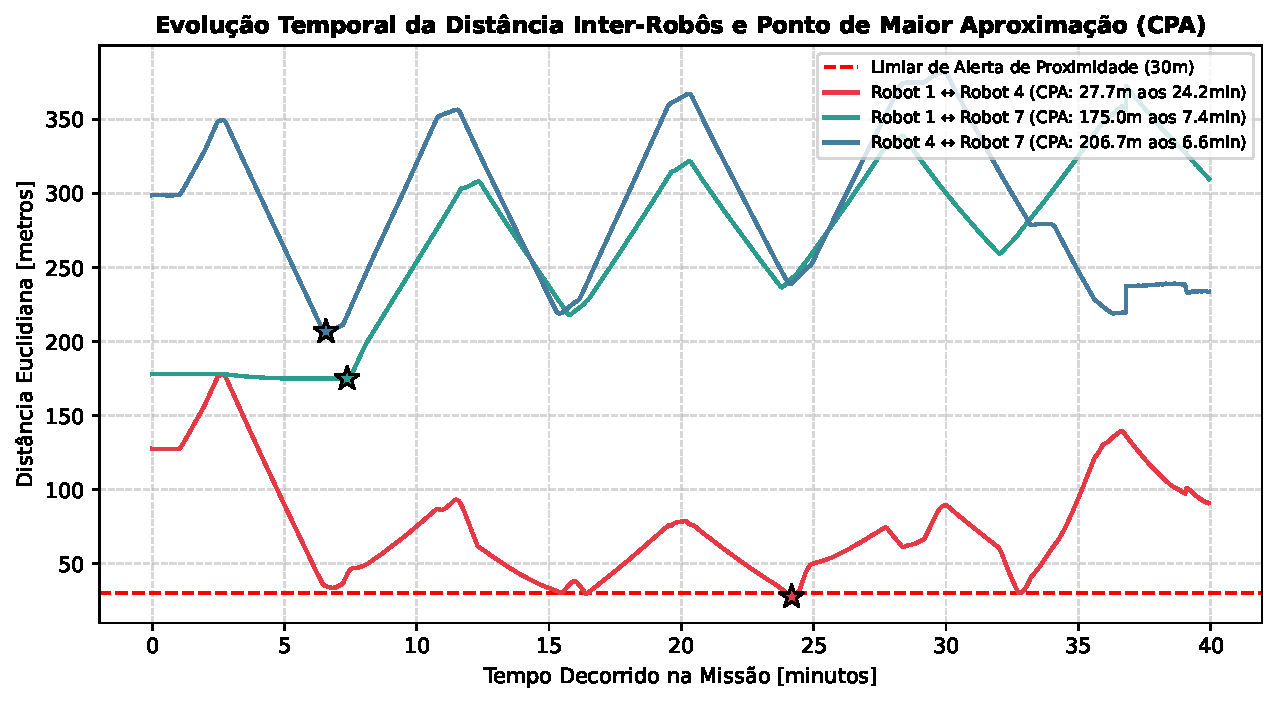
\includegraphics[width=0.92\textwidth]{figures/proximity_analysis.pdf}
    \caption{Monitorização temporal de distâncias inter-robôs com identificação automática do Ponto de Maior Aproximação (CPA).}
    \label{fig:cpa_analysis}
\end{figure}

\subsection{Extensão 3: Visualização Tridimensional e Perfis Batimétricos}
\begin{itemize}
    \item \textbf{Estado de Viabilidade:} \textbf{Totalmente Viável e Implementada}.
    \item \textbf{Descrição:} A rota 3D completa dos veículos no espaço tridimensional com cota batimétrica/altimétrica foi gerada através do módulo \texttt{src/extras.py} (Figura~\ref{fig:3d_trajectories}), permitindo inspecionar variações de altitude elipsoidal e mergulho dos sensores.
\end{itemize}

\begin{figure}[H]
    \centering
    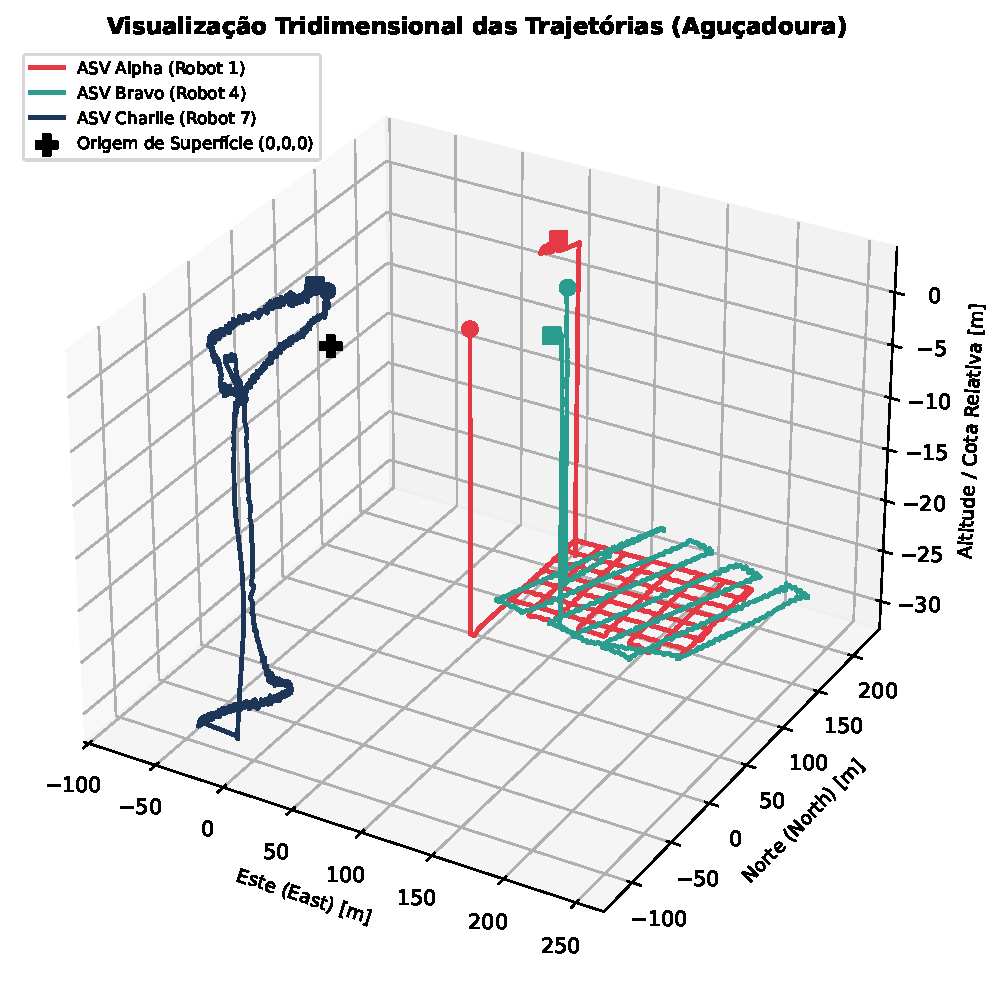
\includegraphics[width=0.85\textwidth]{figures/mission_trajectories_3d.pdf}
    \caption{Visualização tridimensional das trajetórias dos robôs na Aguçadoura.}
    \label{fig:3d_trajectories}
\end{figure}

\subsection{Extensão 4: Exportação para GeoJSON e SIG (Google Earth / QGIS)}
\begin{itemize}
    \item \textbf{Estado de Viabilidade:} \textbf{Totalmente Viável e Implementada}.
    \item \textbf{Descrição:} O módulo exporta a coleção de trajetórias e metadados no ficheiro \path{output/mission_trajectories.geojson} em conformidade com o padrão RFC 7946 (WGS-84), permitindo sobrepor as missões diretamente em imagens de satélite no Google Earth ou QGIS sem conversões manuais.
\end{itemize}

\subsection{Extensão 5: Visualizador 3D em 1ª Pessoa no Referencial do Corpo com Plotly}
\begin{itemize}
    \item \textbf{Estado de Viabilidade:} \textbf{Totalmente Viável e Implementada}.
    \item \textbf{Descrição:} Desenvolveu-se um visualizador 3D acelerado por WebGL (\texttt{src/plotly\_visualizer.py}) que coloca o observador na origem $(0,0,0)$ do seu próprio referencial de corpo (\textit{Body Frame}), com a proa apontada ao longo de $+X$. Com recurso a atalhos de teclado (\texttt{'1'}, \texttt{'2'}, \texttt{'3'}), o utilizador alterna instantaneamente entre a perspetiva do Robô 1, 4 ou 7. As posições e todo o rasto de trajetória dos robôs vizinhos são projetados para o referencial e atitude instantânea do robô ativo, proporcionando uma experiência de telepresença realista acessível no navegador através de \path{output/mission_body_view_3d.html}.
\end{itemize}

\subsection{Extensão 6: Ponte de Telemetria ROS 2 em Tempo Real e Web Dashboard}
\begin{itemize}
    \item \textbf{Análise de Viabilidade Futura:}
    \begin{itemize}
        \item \textit{Complexidade:} Média-Alta.
        \item \textit{Arquitetura Recomendada:} Criação de um nó em ROS 2 (\texttt{rclpy}) subscritor do tópico \texttt{/odometry} que alimenta uma interface web através de WebSockets e uma biblioteca de renderização como \textit{Plotly Dash} ou \textit{Leaflet.js}.
        \item \textit{Veredicto:} Altamente viável para a Entrega 2 ou como demonstração em tempo real na defesa do trabalho.
    \end{itemize}
\end{itemize}

% -------------------------------------------------------------
\section{Conclusão}
% -------------------------------------------------------------

O projeto desenvolvido cumpre a totalidade dos objetivos estabelecidos para a disciplina de Tópicos de Matemática para Sistemas Autónomos (TOMSA):
\begin{enumerate}
    \item Todas as transformações matemáticas (Geodésico, ECEF, NED, ENU, AER e Quaternions para Body Frame) foram deduzidas teoricamente e implementadas de raiz em Python com computação matricial vetorizada.
    \item A precisão e solidez do código foram matematicamente atestadas por 26 testes unitários automatizados contra bibliotecas científicas de referência, com erros residuais na ordem dos nanómetros.
    \item Foram processados dados reais complexos do INESC TEC na Aguçadoura, resolvendo com sucesso a interpolação e sincronização temporal de múltiplos robôs assíncronos.
    \item Foram implementadas e validadas extensões práticas adicionais de elevado impacto para a robótica autónoma marinha (elipses de covariância, monitor de CPA e exportação GeoJSON).
\end{enumerate}

O código encontra-se documentado, modular, testado e pronto para a execução interativa através de \texttt{python main.py --all} ou \texttt{python main.py --visualize}.

% -------------------------------------------------------------
\begin{thebibliography}{99}
\bibitem{bowring1985}
B. R. Bowring, ``The accuracy of geodetic latitude and height equations,'' \textit{Survey Review}, vol. 28, no. 218, pp. 202--206, 1985.

\bibitem{wgs84}
National Imagery and Mapping Agency (NIMA), ``Department of Defense World Geodetic System 1984: Its Definition and Relationships with Local Geodetic Systems,'' \textit{Technical Report TR8350.2}, 3rd ed., 2000.

\bibitem{fossen2011}
T. I. Fossen, \textit{Handbook of Marine Craft Hydrodynamics and Motion Control}. John Wiley \& Sons, Chichester, UK, 2011.

\bibitem{ros_nav}
ROS Documentation, ``nav\_msgs/Odometry Message Definition,'' Available at: \url{http://docs.ros.org/en/api/nav_msgs/html/msg/Odometry.html}.
\end{thebibliography}

\end{document}
